\section{My analysis of the dataset}

According to ChatGPT at the start it is important to describe the dataset in
general, while most of the following information is already given in the
previous section, I will repeat those:
\begin{itemize}
	\item \textbf{Origin of the dataset}: \texttt{rottentomatoes.com}, then
		elaborated by Pang and Lee, the Stanford Parser, Amazon Mechanical Turk.
		Finally three judges were asked to decide on the final sentiment of the
		reviews. Note that the dataset is made of movie reviews;

	\item \textbf{Number of patterns}: 215.154 phrases from 10.662 sentences,
		but they are treated independently;

	\item \textbf{Number of classes}: 5: negative, somewhat negative, neutral,
		somewhat positive, positive. Actually the value given to each sentence
		ranges in 25 classes, but in the paper they are grouped in 5, since the
		most extreme values are not very common. I suppose I will use only 5;

	\item \textbf{Language}: English;
\end{itemize}

\subsection{Labels distribution}

\begin{figure}[H]
	\centering
	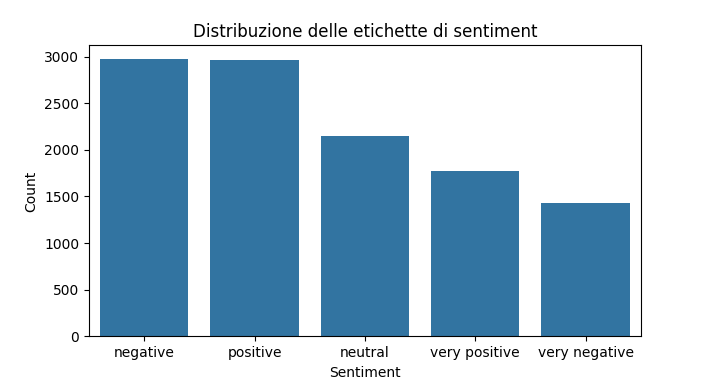
\includegraphics[width=0.8\textwidth]{figures/label_distribution.png}
	\caption{Labels distribution}
	\label{fig:labels_distribution}
\end{figure}

Back to the actual numbers, we got the following distribution:
\begin{itemize}
	\item \textbf{Negative}: 1432;
	\item \textbf{Somewhat negative}: 2971;
	\item \textbf{Neutral}: 2144;
	\item \textbf{Somewhat positive}: 2966;
	\item \textbf{Positive}: 1773;
\end{itemize}

\subsection{Texts length distribution}

\begin{figure}[H]
	\centering
	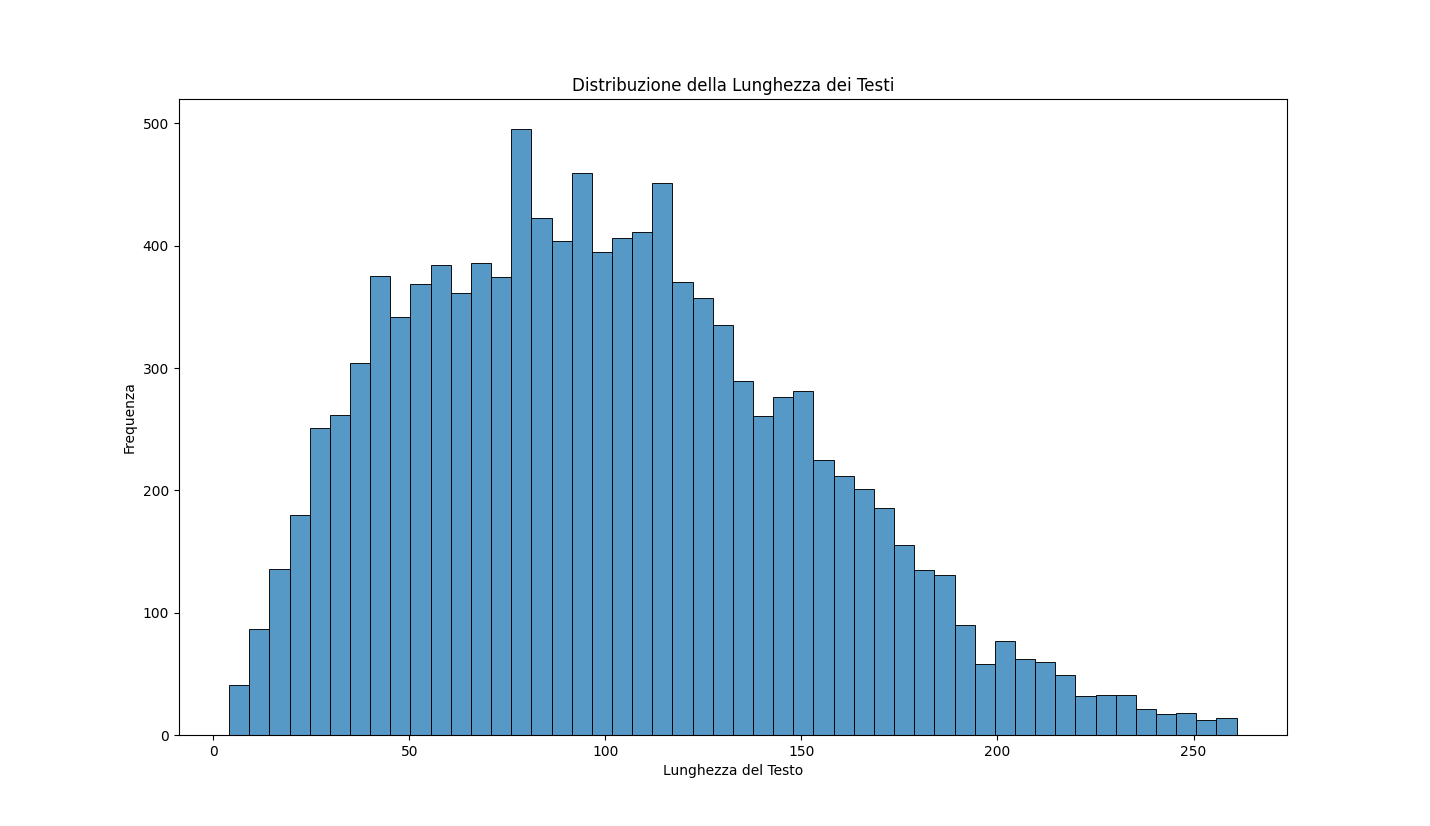
\includegraphics[width=0.8\textwidth]{figures/text_length.png}
	\caption{Texts length distribution}
	\label{fig:text_length_distribution}
\end{figure}

Where the mean of the texts length is 101 and the median is 97.

\subsection{Most frequent words}

\begin{figure}[H]
	\centering
	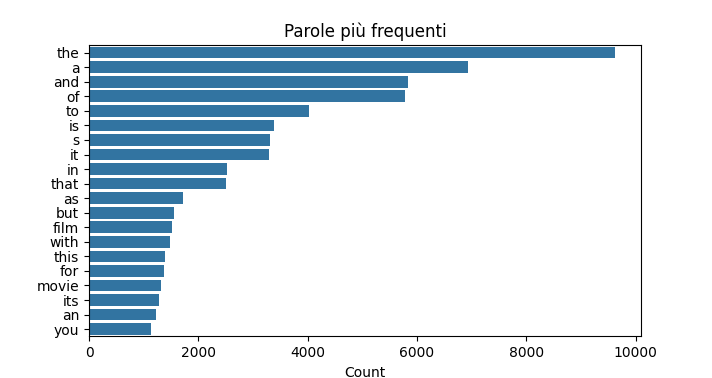
\includegraphics[width=0.8\textwidth]{figures/most_frequent_words.png}
	\caption{Most frequent words}
	\label{fig:most_frequent_words}
\end{figure}

Finally the most frequent words are:
\begin{itemize}
	\item \textbf{the}: 9615;
	\item \textbf{a}: 6934;
	\item \textbf{and}: 5841;
	\item \textbf{of}: 5787;
	\item \textbf{to}: 4033;
\end{itemize}

\subsection{Sentiment visualization}

The sentiment visualization is done through word clouds, where the size of the
word is proportional to the frequency of the word in the dataset, within the
label. The following figures show the word clouds for each label.

\begin{figure}[H]
	\centering
	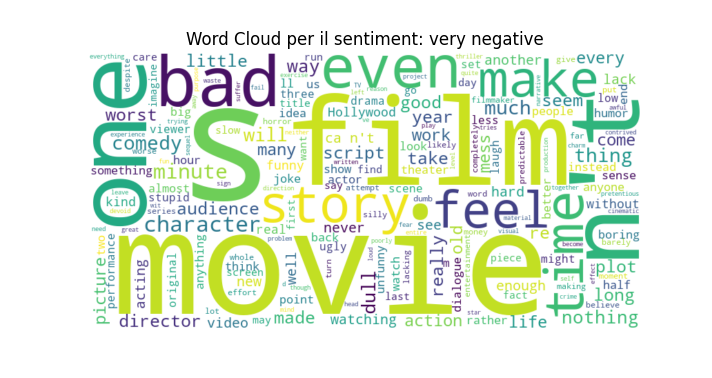
\includegraphics[width=0.8\textwidth]{figures/wordcloud_negative.png}
	\caption{Negative word cloud}
	\label{fig:negative_word_cloud}
\end{figure}

\begin{figure}[H]
	\centering
	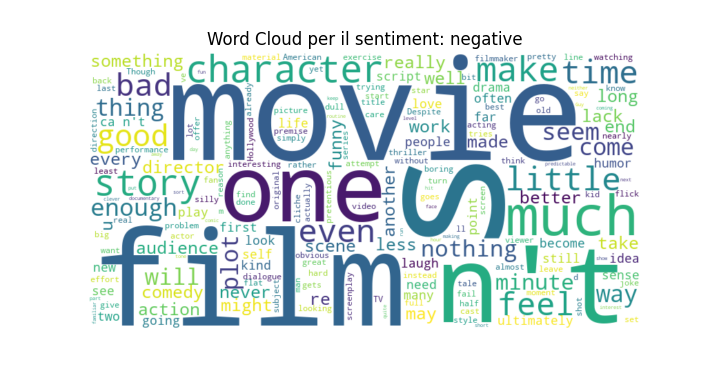
\includegraphics[width=0.8\textwidth]{figures/wordcloud_snegative.png}
	\caption{Somewhat negative word cloud}
	\label{fig:somewhat_negative_word_cloud}
\end{figure}

\begin{figure}[H]
	\centering
	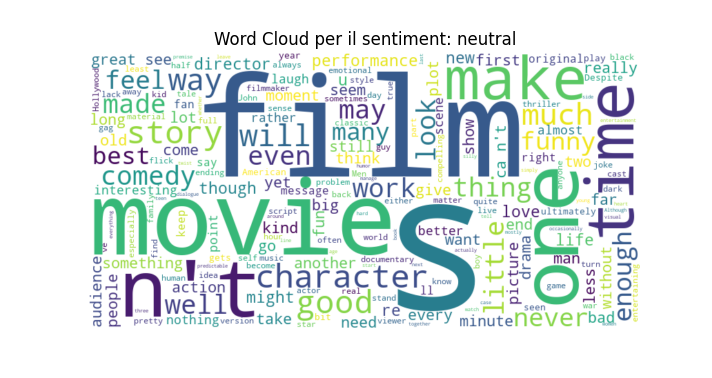
\includegraphics[width=0.8\textwidth]{figures/wordcloud_neutral.png}
	\caption{Neutral word cloud}
	\label{fig:neutral_word_cloud}
\end{figure}

\begin{figure}[H]
	\centering
	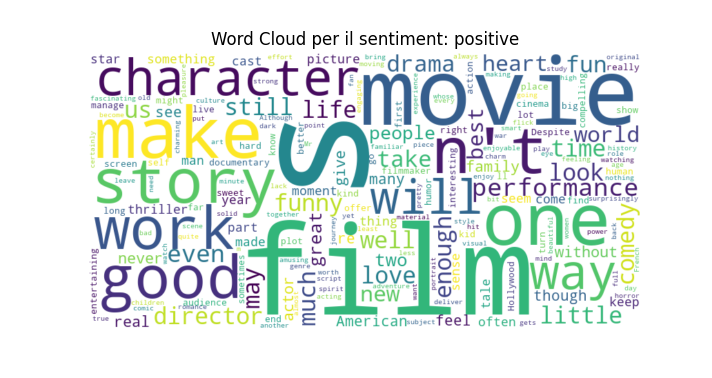
\includegraphics[width=0.8\textwidth]{figures/wordcloud_spositive.png}
	\caption{Somewhat positive word cloud}
	\label{fig:somewhat_positive_word_cloud}
\end{figure}

\begin{figure}[H]
	\centering
	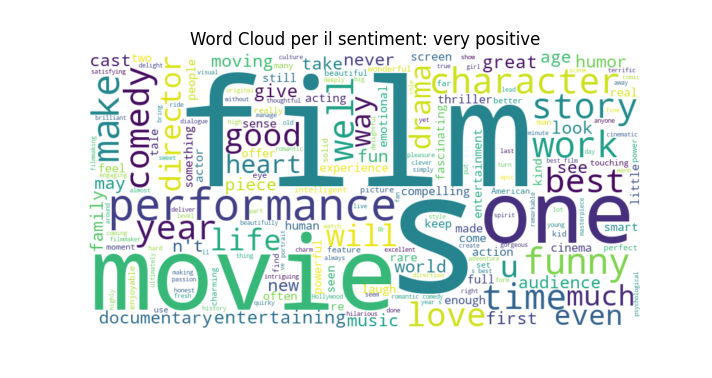
\includegraphics[width=0.8\textwidth]{figures/wordcloud_positive.png}
	\caption{Positive word cloud}
	\label{fig:positive_word_cloud}
\end{figure}
